\documentclass[a4paper, 11pt]{article}

    \usepackage[utf8]{inputenc}
    \usepackage[T1]{fontenc}
    \usepackage{amsmath}
    \usepackage{mathrsfs}
    \usepackage{graphicx}
    \usepackage[top=3cm,left=2cm,bottom=2cm,right=2cm]{geometry}


    \newcommand{\vect}{\overrightarrow}

    \title{Vibrations — Mémo}
    \author{License SPI — S3}
    \date{Novembre 2012}

\begin{document}
    \maketitle

\section{Equation du mouvement linéaire}

\begin{eqnarray*}
    a\ddot{x} + cx = 0 & \Leftrightarrow & \ddot{x} + \frac{c}{a}x = 0\\
                       & \Leftrightarrow & \left\{
    \begin{array}{l}
        \ddot{x} + \omega_0^2~x = 0\\
        \omega_0 = \sqrt{\frac{c}{a}}
    \end{array}
\right.  \end{eqnarray*}

\begin{itemize}
    \item $\omega_0$ : pulsation propre des oscillation libres non-amorties (en $\mathrm{rad}\cdot\mathrm{s}^{-1}$)
\end{itemize}

\section{Solution de l'équation}

$$x(t) = A\cos(\omega_0~t + \phi)$$

\begin{itemize}
    \item $A$ : amplitude du mouvement
    \item $\phi$ : phase
\end{itemize}

\section{Equation du mouvement : pendule circulaire}

$$\ddot{\theta} = \frac{g}{l}\sin\theta = 0$$

Linéarisation de l'équation en utilisant l'approximation harmonique : $\sin\theta\approx\theta$.

\[
    \left\{
    \begin{array}{l}
        \ddot{\theta} + \omega_0^2~\theta = 0\\
        \omega_0 = \sqrt{\frac{g}{l}}
    \end{array}
    \right.
\]

\section{Force de rappel d'un ressort}

\[
    \vect{T} = -k\left(x-l_0\right)\vect{e_x}
\]

\section{Equation du mouvement : Ressort}

\[
    m\ddot{x} + kx = kl_0
\]

\section{PFD pour un solide en rotation sans frottement}

Soit le solide $S$ en rotation autour de l'axe $Oz$. Le point $O$ appartient à l'axe $Oz$.

\[
    \vect{\mathcal{M}_O}(\mathrm{ext} \rightarrow S)\cdot\vect{e_{z_0}} = C\ddot{\theta}
\]

\begin{itemize}
    \item $C$ : moment d'inertie de $S$ autour de $Oz$
\end{itemize}

\section{Moment d'inertie pour une point matériel}

\vfill
\begin{center}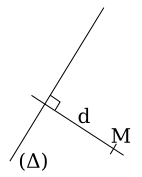
\includegraphics[scale=0.7]{i_delta1.png}\end{center}
\vfill

Le moment d'inertie du point $M$ de masse $m$ s'écrit

\[
    I_\Delta(M,m) = md^2
\]

Pour le moment d'inertie d'un ensemble $\Sigma$ de $n$ points de masses $m_i$ et séparés de la droite d'une distance
$d_i$ :

\[
I_\Delta(\Sigma) = \sum_{i=1}^nm_id_i^2
\]

\section{Théorème de Huygens}

\vfill
\begin{center}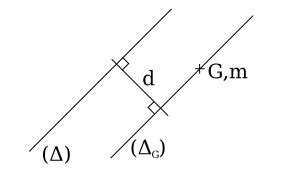
\includegraphics[scale=0.7]{i_delta2.png}\end{center}
\vfill

Soit $G$ le centre de masse d'un solide $S$ (de masse $m$). Connaissant $I_{\Delta_G}(S)$, on peut écrire :

\[
    I_{\Delta}(S) = I_{\Delta_G}(S) + I_\Delta(G,m) = I_{\Delta_G}(S) + md^2
\]

\end{document}
